% Options for packages loaded elsewhere
\PassOptionsToPackage{unicode}{hyperref}
\PassOptionsToPackage{hyphens}{url}
%
\documentclass[
]{article}
\usepackage{amsmath,amssymb}
\usepackage{lmodern}
\usepackage{iftex}
\ifPDFTeX
  \usepackage[T1]{fontenc}
  \usepackage[utf8]{inputenc}
  \usepackage{textcomp} % provide euro and other symbols
\else % if luatex or xetex
  \usepackage{unicode-math}
  \defaultfontfeatures{Scale=MatchLowercase}
  \defaultfontfeatures[\rmfamily]{Ligatures=TeX,Scale=1}
\fi
% Use upquote if available, for straight quotes in verbatim environments
\IfFileExists{upquote.sty}{\usepackage{upquote}}{}
\IfFileExists{microtype.sty}{% use microtype if available
  \usepackage[]{microtype}
  \UseMicrotypeSet[protrusion]{basicmath} % disable protrusion for tt fonts
}{}
\makeatletter
\@ifundefined{KOMAClassName}{% if non-KOMA class
  \IfFileExists{parskip.sty}{%
    \usepackage{parskip}
  }{% else
    \setlength{\parindent}{0pt}
    \setlength{\parskip}{6pt plus 2pt minus 1pt}}
}{% if KOMA class
  \KOMAoptions{parskip=half}}
\makeatother
\usepackage{xcolor}
\usepackage[margin=1in]{geometry}
\usepackage{color}
\usepackage{fancyvrb}
\newcommand{\VerbBar}{|}
\newcommand{\VERB}{\Verb[commandchars=\\\{\}]}
\DefineVerbatimEnvironment{Highlighting}{Verbatim}{commandchars=\\\{\}}
% Add ',fontsize=\small' for more characters per line
\usepackage{framed}
\definecolor{shadecolor}{RGB}{248,248,248}
\newenvironment{Shaded}{\begin{snugshade}}{\end{snugshade}}
\newcommand{\AlertTok}[1]{\textcolor[rgb]{0.94,0.16,0.16}{#1}}
\newcommand{\AnnotationTok}[1]{\textcolor[rgb]{0.56,0.35,0.01}{\textbf{\textit{#1}}}}
\newcommand{\AttributeTok}[1]{\textcolor[rgb]{0.77,0.63,0.00}{#1}}
\newcommand{\BaseNTok}[1]{\textcolor[rgb]{0.00,0.00,0.81}{#1}}
\newcommand{\BuiltInTok}[1]{#1}
\newcommand{\CharTok}[1]{\textcolor[rgb]{0.31,0.60,0.02}{#1}}
\newcommand{\CommentTok}[1]{\textcolor[rgb]{0.56,0.35,0.01}{\textit{#1}}}
\newcommand{\CommentVarTok}[1]{\textcolor[rgb]{0.56,0.35,0.01}{\textbf{\textit{#1}}}}
\newcommand{\ConstantTok}[1]{\textcolor[rgb]{0.00,0.00,0.00}{#1}}
\newcommand{\ControlFlowTok}[1]{\textcolor[rgb]{0.13,0.29,0.53}{\textbf{#1}}}
\newcommand{\DataTypeTok}[1]{\textcolor[rgb]{0.13,0.29,0.53}{#1}}
\newcommand{\DecValTok}[1]{\textcolor[rgb]{0.00,0.00,0.81}{#1}}
\newcommand{\DocumentationTok}[1]{\textcolor[rgb]{0.56,0.35,0.01}{\textbf{\textit{#1}}}}
\newcommand{\ErrorTok}[1]{\textcolor[rgb]{0.64,0.00,0.00}{\textbf{#1}}}
\newcommand{\ExtensionTok}[1]{#1}
\newcommand{\FloatTok}[1]{\textcolor[rgb]{0.00,0.00,0.81}{#1}}
\newcommand{\FunctionTok}[1]{\textcolor[rgb]{0.00,0.00,0.00}{#1}}
\newcommand{\ImportTok}[1]{#1}
\newcommand{\InformationTok}[1]{\textcolor[rgb]{0.56,0.35,0.01}{\textbf{\textit{#1}}}}
\newcommand{\KeywordTok}[1]{\textcolor[rgb]{0.13,0.29,0.53}{\textbf{#1}}}
\newcommand{\NormalTok}[1]{#1}
\newcommand{\OperatorTok}[1]{\textcolor[rgb]{0.81,0.36,0.00}{\textbf{#1}}}
\newcommand{\OtherTok}[1]{\textcolor[rgb]{0.56,0.35,0.01}{#1}}
\newcommand{\PreprocessorTok}[1]{\textcolor[rgb]{0.56,0.35,0.01}{\textit{#1}}}
\newcommand{\RegionMarkerTok}[1]{#1}
\newcommand{\SpecialCharTok}[1]{\textcolor[rgb]{0.00,0.00,0.00}{#1}}
\newcommand{\SpecialStringTok}[1]{\textcolor[rgb]{0.31,0.60,0.02}{#1}}
\newcommand{\StringTok}[1]{\textcolor[rgb]{0.31,0.60,0.02}{#1}}
\newcommand{\VariableTok}[1]{\textcolor[rgb]{0.00,0.00,0.00}{#1}}
\newcommand{\VerbatimStringTok}[1]{\textcolor[rgb]{0.31,0.60,0.02}{#1}}
\newcommand{\WarningTok}[1]{\textcolor[rgb]{0.56,0.35,0.01}{\textbf{\textit{#1}}}}
\usepackage{graphicx}
\makeatletter
\def\maxwidth{\ifdim\Gin@nat@width>\linewidth\linewidth\else\Gin@nat@width\fi}
\def\maxheight{\ifdim\Gin@nat@height>\textheight\textheight\else\Gin@nat@height\fi}
\makeatother
% Scale images if necessary, so that they will not overflow the page
% margins by default, and it is still possible to overwrite the defaults
% using explicit options in \includegraphics[width, height, ...]{}
\setkeys{Gin}{width=\maxwidth,height=\maxheight,keepaspectratio}
% Set default figure placement to htbp
\makeatletter
\def\fps@figure{htbp}
\makeatother
\setlength{\emergencystretch}{3em} % prevent overfull lines
\providecommand{\tightlist}{%
  \setlength{\itemsep}{0pt}\setlength{\parskip}{0pt}}
\setcounter{secnumdepth}{-\maxdimen} % remove section numbering
\usepackage{float} \floatplacement{figure}{H}
\ifLuaTeX
  \usepackage{selnolig}  % disable illegal ligatures
\fi
\IfFileExists{bookmark.sty}{\usepackage{bookmark}}{\usepackage{hyperref}}
\IfFileExists{xurl.sty}{\usepackage{xurl}}{} % add URL line breaks if available
\urlstyle{same} % disable monospaced font for URLs
\hypersetup{
  pdftitle={Peas Out Rob},
  pdfauthor={Rob Clark \& Riley Anderson},
  hidelinks,
  pdfcreator={LaTeX via pandoc}}

\title{Peas Out Rob}
\author{Rob Clark \& Riley Anderson}
\date{October 09, 2023}

\begin{document}
\maketitle

{
\setcounter{tocdepth}{2}
\tableofcontents
}
\hypertarget{overview}{%
\subsection{Overview}\label{overview}}

This analysis explores Rob Clark's ``Peas Out'' data.

\hypertarget{experimental-design}{%
\subsection{Experimental Design}\label{experimental-design}}

24 bug dorms (2m x 2m x 2m) were established on an experimental farm
plot that was sown with banner pea. The dorms were laid out in a square
design with 8 control dorms in the center. Control dorms were flanked by
2 sides (4 dorms/side) where common vetch was planted in the distal half
(the outer circumference of the square) and banner pea was planted in
the proximal half (the inner circumference of the square). Diagonally
from the vetch dorms were 2 sides similarly planted with red clover.

\begin{Shaded}
\begin{Highlighting}[]

\NormalTok{knitr}\SpecialCharTok{::}\FunctionTok{include\_graphics}\NormalTok{(}\StringTok{"images/peas.out.design.png"}\NormalTok{, }\AttributeTok{error =} \ConstantTok{FALSE}\NormalTok{)}
\end{Highlighting}
\end{Shaded}

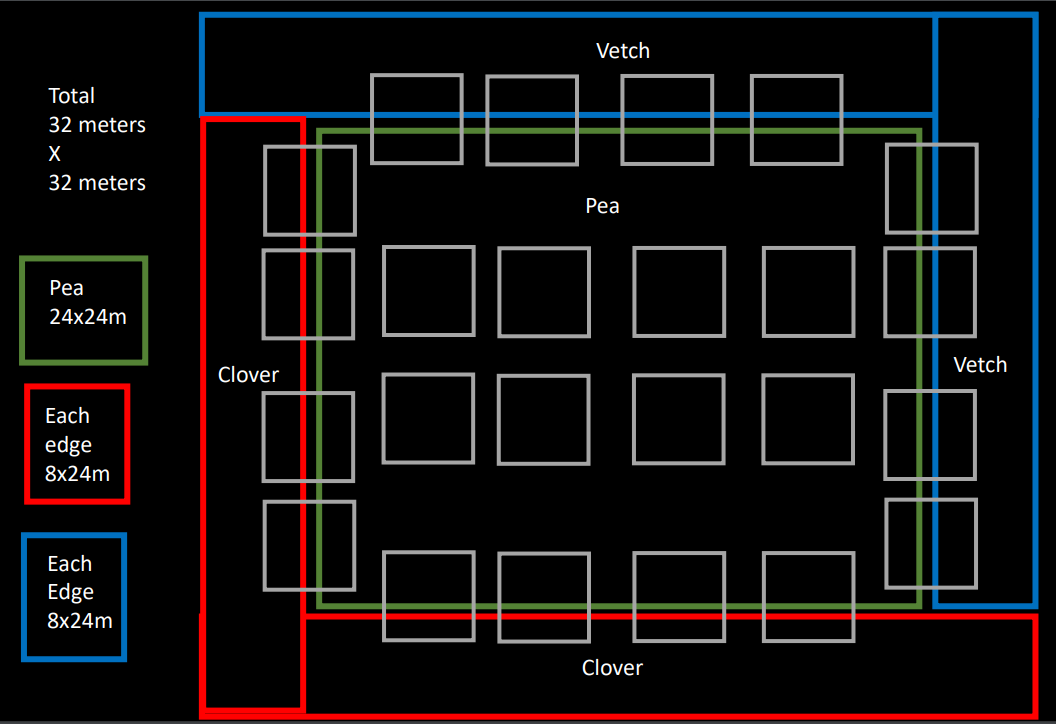
\includegraphics{images/peas.out.design.png}

\hypertarget{summary-of-results}{%
\subsubsection{Summary of Results}\label{summary-of-results}}

\begin{itemize}
\tightlist
\item
\end{itemize}

\hypertarget{session-information}{%
\subsection{Session Information}\label{session-information}}

\begin{verbatim}
R version 4.2.3 (2023-03-15 ucrt)
Platform: x86_64-w64-mingw32/x64 (64-bit)
Running under: Windows 10 x64 (build 19045)

Matrix products: default

locale:
[1] LC_COLLATE=English_United States.utf8 
[2] LC_CTYPE=English_United States.utf8   
[3] LC_MONETARY=English_United States.utf8
[4] LC_NUMERIC=C                          
[5] LC_TIME=English_United States.utf8    

attached base packages:
[1] stats     graphics  grDevices utils     datasets  methods   base     

other attached packages:
 [1] sjPlot_2.8.13      glmmTMB_1.1.6      multcompView_0.1-9 piecewiseSEM_2.3.0
 [5] MuMIn_1.47.5       emmeans_1.8.5      lubridate_1.9.2    forcats_1.0.0     
 [9] stringr_1.5.0      dplyr_1.1.1        purrr_1.0.1        readr_2.1.4       
[13] tidyr_1.3.0        tibble_3.2.1       ggplot2_3.4.1      tidyverse_2.0.0   
[17] multcomp_1.4-23    TH.data_1.1-2      MASS_7.3-58.2      survival_3.5-3    
[21] mvtnorm_1.1-3      car_3.1-2          carData_3.0-5      lme4_1.1-32       
[25] Matrix_1.6-1      

loaded via a namespace (and not attached):
 [1] jsonlite_1.8.4      splines_4.2.3       modelr_0.1.11      
 [4] datawizard_0.7.0    highr_0.10          stats4_4.2.3       
 [7] bayestestR_0.13.0   yaml_2.3.7          backports_1.4.1    
[10] numDeriv_2016.8-1.1 pillar_1.9.0        lattice_0.20-45    
[13] glue_1.6.2          digest_0.6.31       RColorBrewer_1.1-3 
[16] minqa_1.2.5         colorspace_2.1-0    sandwich_3.0-2     
[19] htmltools_0.5.5     pkgconfig_2.0.3     broom_1.0.4        
[22] DiagrammeR_1.0.10   xtable_1.8-4        scales_1.2.1       
[25] tzdb_0.3.0          timechange_0.2.0    generics_0.1.3     
[28] sjlabelled_1.2.0    withr_2.5.0         TMB_1.9.2          
[31] cli_3.6.1           magrittr_2.0.3      estimability_1.4.1 
[34] evaluate_0.20       fansi_1.0.4         nlme_3.1-162       
[37] tools_4.2.3         hms_1.1.3           lifecycle_1.0.3    
[40] munsell_0.5.0       ggeffects_1.2.0     compiler_4.2.3     
[43] rlang_1.1.0         grid_4.2.3          nloptr_2.0.3       
[46] rstudioapi_0.14     htmlwidgets_1.6.2   visNetwork_2.1.2   
[49] rmarkdown_2.21      boot_1.3-28.1       gtable_0.3.3       
[52] codetools_0.2-19    sjstats_0.18.2      abind_1.4-5        
[55] sjmisc_2.8.9        R6_2.5.1            zoo_1.8-12         
[58] knitr_1.42          performance_0.10.2  fastmap_1.1.1      
[61] utf8_1.2.3          rprojroot_2.0.3     insight_0.19.1     
[64] stringi_1.7.12      Rcpp_1.0.10         vctrs_0.6.1        
[67] tidyselect_1.2.0    xfun_0.38          
\end{verbatim}

\end{document}
